% !TeX TS-program = latexmk --lualatex

\documentclass[aspectratio=169]{beamer}

\usepackage{tikzlings}

\setbeamertemplate{navigation symbols}{}
\setbeamertemplate{background canvas}{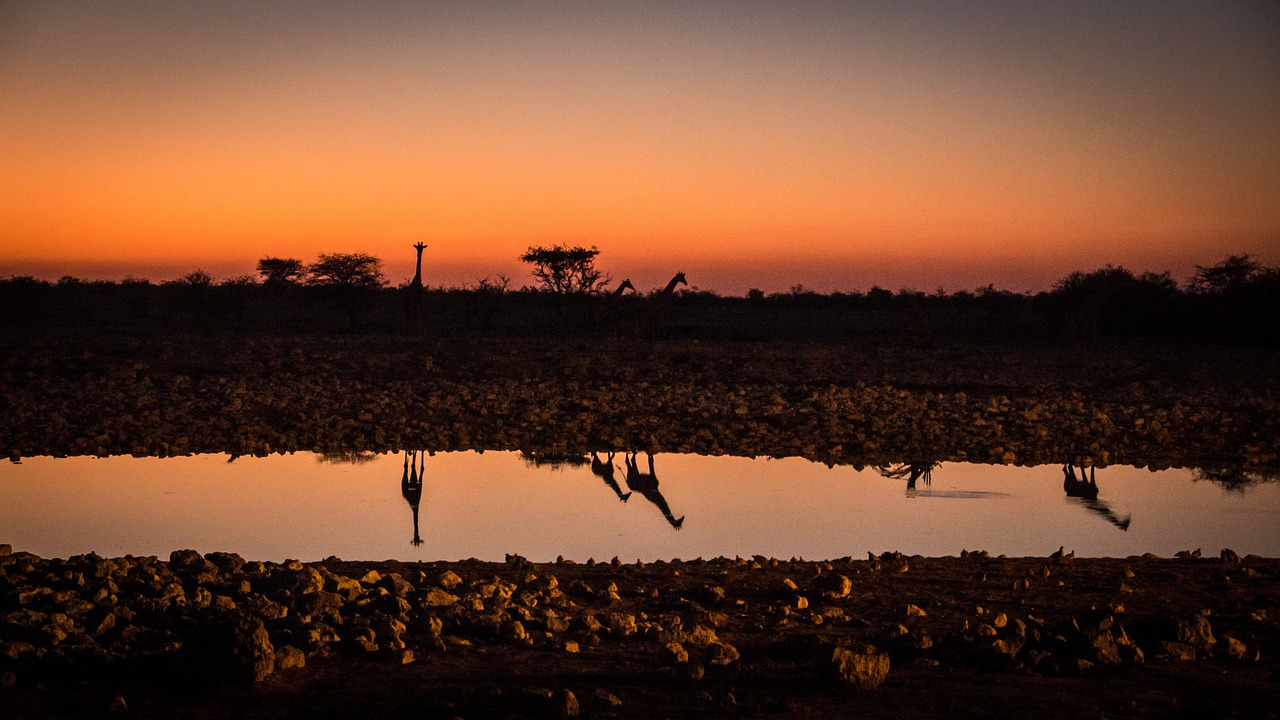
\includegraphics[width=\paperwidth]{namibia-2949409_1280}}
\graphicspath{{include/}}

% trick taken from https://topanswers.xyz/tex?q=1989
\tikzset{
    use page relative coordinates/.style={
        shift={(current page.south west)},
        x={(current page.south east)},
        y={(current page.north west)}
    },
}

\usepackage{xfp}
\ExplSyntaxOn
\let\intmodnn\int_mod:nn
\ExplSyntaxOff

\makeatletter
\newcommand{\hippohookbody}{
\ifnum \intmodnn{\thepage}{20} > 10
  \filldraw[\hippo@mouth,line width=\scalingfactor*0.4pt] (0.125, 1.5) arc [start angle=-50, end angle=-130, radius=0.2] -- cycle;
\fi
}
\makeatother

\newcommand{\isopen}{%
\ifnum \intmodnn{\thepage}{20} > 10
  -open
\fi
}

\usepackage{fontspec}
\newfontfamily{\african}{African}

\begin{document}

\begin{frame}
  \begin{tikzpicture}[remember picture, overlay]
  
    \hippo[body=gray!70!black,      eye=darkgray!61!white,scale=2.5,yshift=-2cm,xshift=5.25cm]
    
    \node[rotate=-5*sin(\thepage*3),anchor=south] at (1,-1.5) {
\includegraphics[page=1,height=1cm]{color-elefant}};
    \node[rotate=-5*sin(\thepage*3),anchor=south] at (4,-1.5) {
\includegraphics[page=1,height=1cm]{color-meerkat}};
    \node[rotate=-5*sin(\thepage*3),anchor=south] at (7,-1.5) {
\includegraphics[page=1,height=1cm]{color-ape}};
    \node[rotate=-5*sin(\thepage*3),anchor=south] at (10,-1.5) {
\includegraphics[page=1,height=1cm]{color-rhino}};

    % credit for background image
    \node[white,text width=.7\paperwidth,font=\tiny,align=center] at ([yshift=0.35cm]current page.south) {Image by @manuzoli (\url{https://pixabay.com/photos/namibia-wildlife-africa-etosha-2949409/})};

  \end{tikzpicture}
  \pause[150]
\end{frame}

\def\steps{90}
\begin{frame}
  \begin{tikzpicture}[remember picture, overlay]
    
    \hippo[body=gray!70!black,      eye=darkgray!61!white,scale=2.5,yshift=-2cm,xshift=5.25cm]
    
    \node[rotate=-5*sin(\thepage*3),anchor=south,scale=1+2*\insertoverlaynumber/\steps] at (1,-1.5-0.04*\insertoverlaynumber) {
\includegraphics[page=\insertoverlaynumber,height=1cm]{color-elefant}};
    \node[rotate=-5*sin(\thepage*3),anchor=south,scale=1+2*\insertoverlaynumber/\steps] at (4,-1.5-0.04*\insertoverlaynumber) {
\includegraphics[page=\insertoverlaynumber,height=1cm]{color-meerkat}};
    \node[rotate=-5*sin(\thepage*3),anchor=south,scale=1+2*\insertoverlaynumber/\steps] at (7,-1.5-0.04*\insertoverlaynumber) {
\includegraphics[page=\insertoverlaynumber,height=1cm]{color-ape}};
    \node[rotate=-5*sin(\thepage*3),anchor=south,scale=1+2*\insertoverlaynumber/\steps] at (10,-1.5-0.04*\insertoverlaynumber) {
\includegraphics[page=\insertoverlaynumber,height=1cm]{color-rhino}};    
       
    % credit for background image
    \node[white,text width=.7\paperwidth,font=\tiny,align=center] at ([yshift=0.35cm]current page.south) {Image by @manuzoli (\url{https://pixabay.com/photos/namibia-wildlife-africa-etosha-2949409/})};

  \end{tikzpicture}
  \pause[\steps]
\end{frame}


\begin{frame}
  \begin{tikzpicture}[remember picture, overlay]
    
    \hippo[body=gray!70!black,      eye=darkgray!61!white,scale=2.5,yshift=-2cm,xshift=5.25cm]
    
    \node[rotate=-5*sin(\thepage*3),anchor=south,scale=1+2] at (1,-1.5-0.04*\steps) {
\includegraphics[page=\steps,height=1cm]{color-elefant}};
    \node[rotate=-5*sin(\thepage*3),anchor=south,scale=1+2] at (4,-1.5-0.04*\steps) {\includegraphics[page=\steps,height=1cm]{color-meerkat\isopen}};
    \node[rotate=-5*sin(\thepage*3),anchor=south,scale=1+2] at (7,-1.5-0.04*\steps) {\includegraphics[page=\steps,height=1cm]{color-ape\isopen}};
    \node[rotate=-5*sin(\thepage*3),anchor=south,scale=1+2] at (10,-1.5-0.04*\steps) {\includegraphics[page=\steps,height=1cm]{color-rhino\isopen}};
               
    % credit for background image
    \node[white,text width=.7\paperwidth,font=\tiny,align=center] at ([yshift=0.35cm]current page.south) {Image by @manuzoli (\url{https://pixabay.com/photos/namibia-wildlife-africa-etosha-2949409/})};

  \end{tikzpicture}
  \pause[300]
\end{frame}

\begin{frame}[label=text]
\begin{tikzpicture}[remember picture,overlay]
  \fill[black!90!white] (current page.south west) rectangle (current page.north east);
  \node[text width=.9\linewidth,yellow,align=center] at (current page.center) {\african\fontsize{40}{62}\selectfont Meanwhile\space\space\space\space\space in the\space\space\space\space\space lion\space\space\space\space\space ca\kern-0.1em ve\par}; 
\end{tikzpicture}
\pause[75]
\end{frame}

\begin{frame}
\begin{tikzpicture}[remember picture,overlay,inner sep=0pt]
\node[anchor=west] at (current page.west) {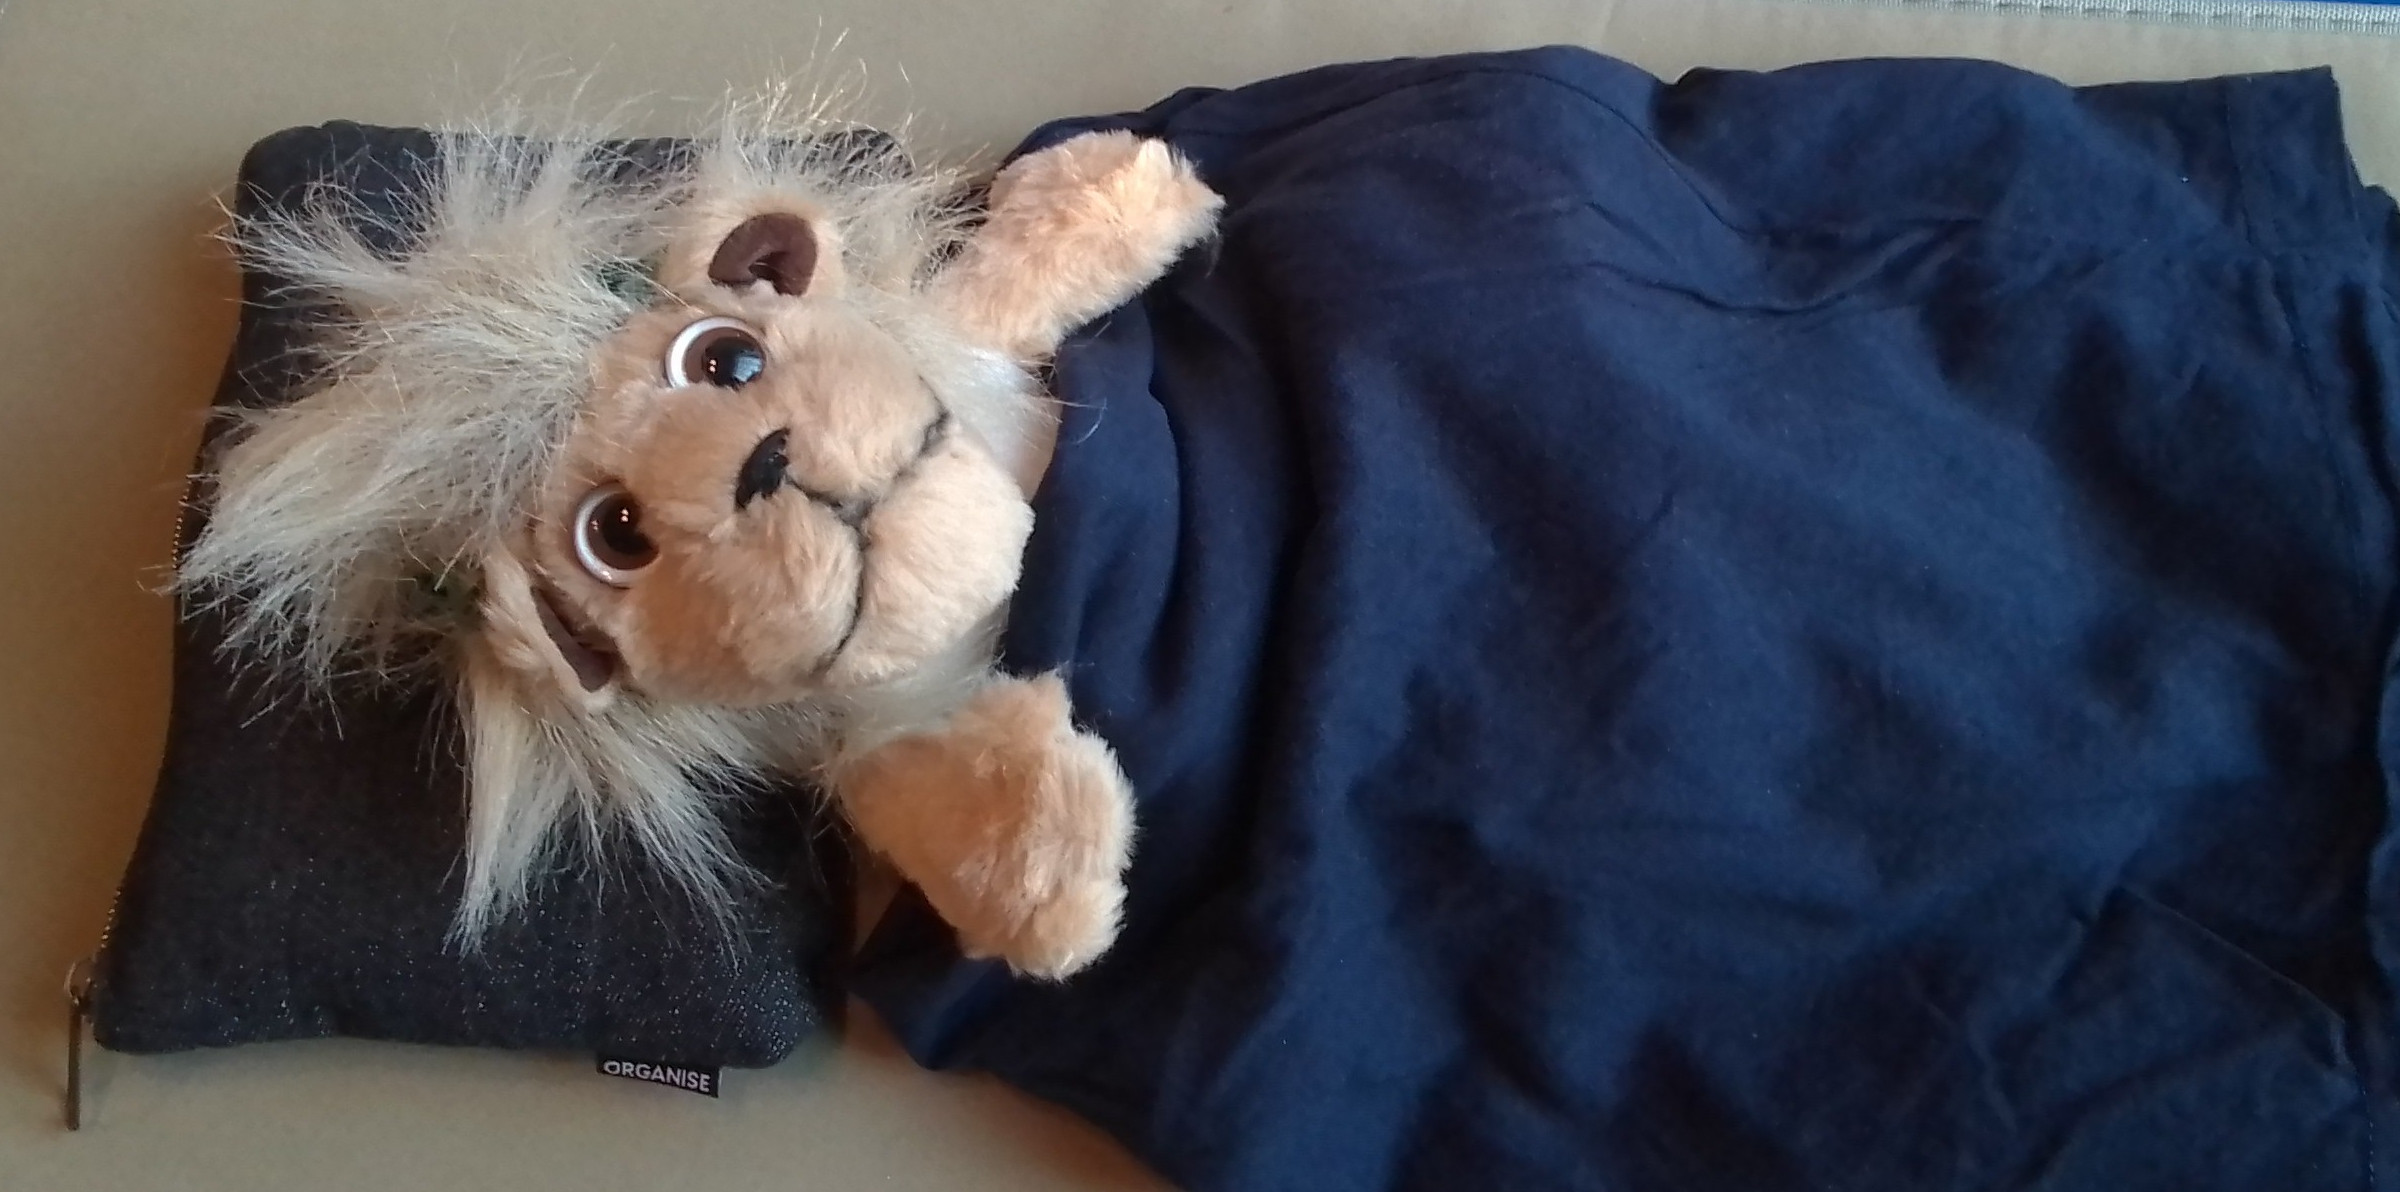
\includegraphics[height=\paperheight]{IMG_20241130_152044}};
\node[anchor=west] at (current page.west) {
\includegraphics[height=\paperheight]{sleepmask}};
\pause[225]
\end{tikzpicture}
\end{frame}

\end{document}